%\section{Design overview}
% Consider making this a chapter of its own
\section{How the three step plan got formulated}
It became obvious from the beginning of this project that there were different ways to go about solving this path finding problem. One of the first realizations that arose was the similarity of this problem with the traveling salesman problem. Both problems were about visiting certain number of nodes before returning to the start node; in the travelings salesman problem the nodes represent cities and in this problem the nodes represent rooms. This would serve as the starting point of the thesis. The question would later be how to go about representing the places that the robot had to visit. An obvious solution was to have a graph where the nodes represent rooms and the edges would represent the connection to those rooms [insert picture of simple graph].

\begin{figure}[H]
    \centering
    \includegraphics[width=1\textwidth]{fig/report/tilhørende_tsp_solution.png}
    \label{}
    \caption[Design overview]{}
\end{figure}

This simple representation would have a few challenges associated with it, the main one being that a straight line between two room nodes would not model very well the real connection between the two rooms. Spot would not be able to walk in a straight line from one room to another because there would be walls blocking the path. 
The graph therefore needed to have a little more information, so door nodes and corner nodes were added. The door nodes would be the only nodes that could cross walls. The job of the corner nodes would be to act as a concave point i.e a point that would be placed at 90 degree or more corners. With this information the first basic solution to the problem could be made. [insert basic solution to the problem].
\begin{figure}[H]
    \centering
    \includegraphics[width=1\textwidth]{fig/report/tsp_solution_med_mange_døre.png}
    \label{}
    \caption[Design overview]{}
\end{figure}

The issue now was to account for the dimensions of the robot in the graph. So far it would only be represented as a point with radius 0. Accounting for the dimensions would show itself to be one of the main challenges of this project. 
The same way that when people walk around in a building they don't walk right next to the wall, scraping their shoulder to the wall (unless the path is very narrow) the same should be the case for the robot. If there was no buffer zone in front of the walls of the building, one could imagine that when Spot would have to turn a corner the program would tell it to walk right alongside the wall since this would allow for the shortest path to turn the corner.


It became clear that some form of discretization would have to take place to indicate exactly where Spot could be and where it could not be.
The question was whether to discretize the entire map or discretize just the route.
% Analysis
%\section{Grid data vs visibility graph}
%To make the robot walk from one room to another or one place in the building to another, it is important to understand  and decide on a way to implement the connectivity between the rooms. There are mainly two different kinds of implementations; a graph connectivity implementation and a grid implementation.
%\\\\
%The grid implementation works by discretizing the floor of the building into a grid with nodes of a specific size; the smaller the node size the higher the resolution of the grid.
%\\
%The graph connectivity approach works by representing each room/area by a node/dot which will be connected by a line to other rooms in the floor.

%The different implementations have different advantages and limitations. For example computationally the graph connectivity approach is much more scalable with bigger buildings or construction sites where as implementing a grid system in these situations will be more taxing computationally since a lot of nodes will have to be calculated. 

%On the other hand the advantage of the grid method is that its pathfinding algorithms will work on all building shapes. 
%Imagine the floor plan of the building below:


%When using a grid system apporach it will be possible to get an agent to walk from area 12 to 13 by specifically telling it which nodes are walkable and which nodes are not e.g walls. This will not be possible for the graph connectivity graph. The graph will here see only that area 12 and 13 are connected but not in which way. The method will draw a straight line between the two points and not see that the areas in reality are connected by the long pathway that goes through the entire floor plan.
% End Analysis

\subsection{Map disretization / distance field}
One way to solve this challenge is to discretize the entire map and for each cell find the distance to the nearest wall. If the distance from the wall to the cell is smaller than the radius of the robot, the cell will be deemed not traversable since this means that the robot will hit the wall. If the distance to the wall is larger than the radius the cell is traversable. What we get by doing this is a Boolean distance field. Where we have nodes that are traversable and nodes that are not.

  

\begin{figure}[H]
    \centering
    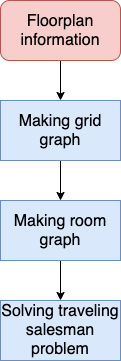
\includegraphics[width=0.4\textwidth]{fig/report/big_structure.png}
    \label{}
    \caption[Design overview]{}
\end{figure}

The issue with this approach is that the number of nodes is directly proportional to the size of the building. For bigger buildings this might cause a problem with performance of the program. 
With that said the distance field allows for certain advantages that makes it a very robust solution. It is a robust solution because it for all nodes in the grid indicates whether Spot can traverse the node or not. This makes the approach useful for all kinds of obscure buildings.
%The advantage of this approach is that it is easy and a straightforward way to tell the robot which nodes it is allowed to traverse which it can not. %This  
%It is also fast to look up because you have done the preprocessing before hand.
Another pro of this approach is that it will be beneficial when we later want to find optimal node placements in the rooms we are visiting. This is because the rooms will already be discretized which makes generating room nodes a simpler process.


\subsection{Route discretization}
Another way to go about the problem would be to discretize the route. The implementation of this would be a bit more complicated but would be rewarded by its scalability to bigger buildings. 
The idea here is to only discretize the route that the robot will walk instead of discretizing the entire map. 
%This could be done in different ways.
One heuristic to this could be that along the route Spot will check if it is near a wall using a distance function. The interval here can be dynamic e.g if the distance to the nearest wall is 5 meters and the radius of the robot is 1 meter it can walk for 4 meter without hitting a wall.
This means that between two nodes - a start and an end node - a lot more nodes will be placed. The robot will go to a node find the distance to the nearest wall and then walk in a straight line towards the node it is seeking the same amount as the distance to the nearest wall minus the radius. Then it will check again to see what the distance to the nearest wall is and repeat the process. It is important that the room/end nodes are a certain radius away from the walls to begin with. 

%One way to go about this is to check the distance to all the walls for every node. This does not scale very well when the number of walls increases. 
%Another way is to have a certain datastructure that takes all the walls and find the nearest quickly.

%One other problem with discretizing the route is that a large percentage of the time the obstacle between 2 room nodes are walls and this means that this A star algorithm will often fail, since the only way to walk through walls are using the doors. 
\\\\
In the end discretization of the entire map was chosen with the thought in mind that the program is not in real-time and therefore fast performance is not a requirement. Implementation wise the distance field would also be a more robust solution and easier to implement. With the route discretization a lot of different worst case scenarios would have to be accounted for and considered, while this would not be the case with the distance field since the program tells Spot very precisely which nodes it can traverse and which it can not. The distance field might also be a better implementation long term since it can allow for certain algorithms when placing the room nodes, explained further in \ref{k_means}.  
\\\\
Representing the building with a graph that would both allow for paths that would not traverse through walls and also allow for the dimensions of Spot, was only one part of the program. Now we would have to figure out how to solve the traveling salesman problem from there.

Looking at the approximate solutions for the TSP the minimum spanning tree of a complete graph was needed. 
Therefore what needed to be done was to make a complete graph that only consisted of the room nodes i.e the nodes that would have to be visited.  
When having that the TSP solution for the "room" graph could be found and that could be translated to the grid graph.
\\
Looking at the flowchart below this overall structure is seen. We first start by making the grid graph, that allows for legal paths and allows for the dimension of the robot. From that graph the program then constructs a room graph that is complete i.e there is an edge between all the room nodes. At last the program solves the approximate TSP for the building.

\begin{figure}[H]
    \centering
    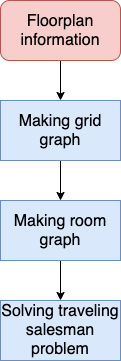
\includegraphics[width=0.4\textwidth]{fig/report/big_structure.png}
    \label{}
    \caption[Design overview]{}
\end{figure}




\section{Making the grid graph}
Looking at the figure below the flowchart of how the grid graph is generated is given. Making the grid graph we would need to sample the building with a given resolution and place a node on each sample and connecting nodes that are next to each other and diagonal to each other with edges. We would end up with a very dense and big graph. The usefulness of the grid graph is that it can have nodes that Spot can traverse and nodes that it can not traverse. Essentially the non traversable nodes are the ones near the walls - the nodes outside the building is also removed later in the program. Therefore a buffer zone between the walls of the building and the open space area is desired. We therefore need to remove the nodes that are within a certain distance of the nearest wall. For that reason the spatial data structure is made for the lines, such that the distance for each node to the closest line can be evaluated. The spatial data structure for the rooms are also made and the same for the nodes. The data structure for the rooms will become useful when making the room graph and so will the data structure for the nodes.

\begin{figure}[H]
    \centering
    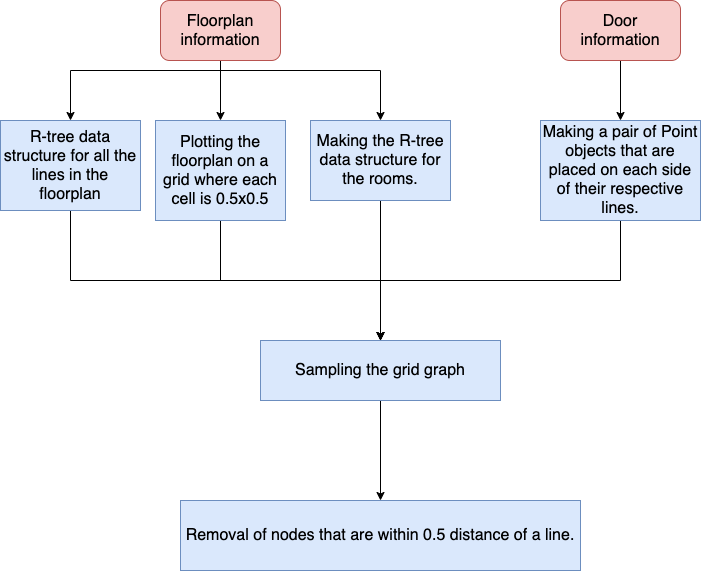
\includegraphics[width=1\textwidth]{fig/report/making_grid_graph.png}
    \label{}
    \caption[Design overview]{}
\end{figure}


\section{Making the room graph}
As explained before, after having made the grid graph, the program needs to make the room graph that needs to be complete. This is because we want to have a graph that only consists of the room nodes such that we can get an approximate TSP solution on that graph. The reason it needs to be complete is that Spot needs to be able to visit each room node from each other room node. This is needed to find the approximate solution of the TSP problem. If there are room nodes that for one reason or another can not be connected to the rest of the room nodes, they are removed from the graph, since this mean that they can not be visited by Spot.

To make the room graph the program needs to first generate the room nodes. Before the program can do that it needs to figure out which rooms each node belongs to, since it is not possible to generate nodes in all rooms with certainty if the program can not distinguish between the rooms. Therefore it first does the room labeling heuristic, which makes use of the ray casting algorithm. This is also where outside nodes are removed from the graph, since they are not part of any room.

When each node has been successfully labeled with a room number, it is time to generate the room nodes. Generating the room nodes were also one of the big discussion points of the project with a few alternative solutions available.
% From Analysis 
\section{Optimal placement of nodes}
The program needs a way to figure out where to place the "room" nodes. Ideally we want to have the "room" nodes placed in such a way that the robot can do point scans of the entire room. Different approaches can be taken to solve this challenge. 

The simplest idea would be to make a bounding rectangle of the room and place a node in the middle of that room. This would work on a lot of rooms that are already square shaped but there would be a risk of a node being placed outside the room for non convex shaped rooms. 
\begin{figure}[H]
    \centering
    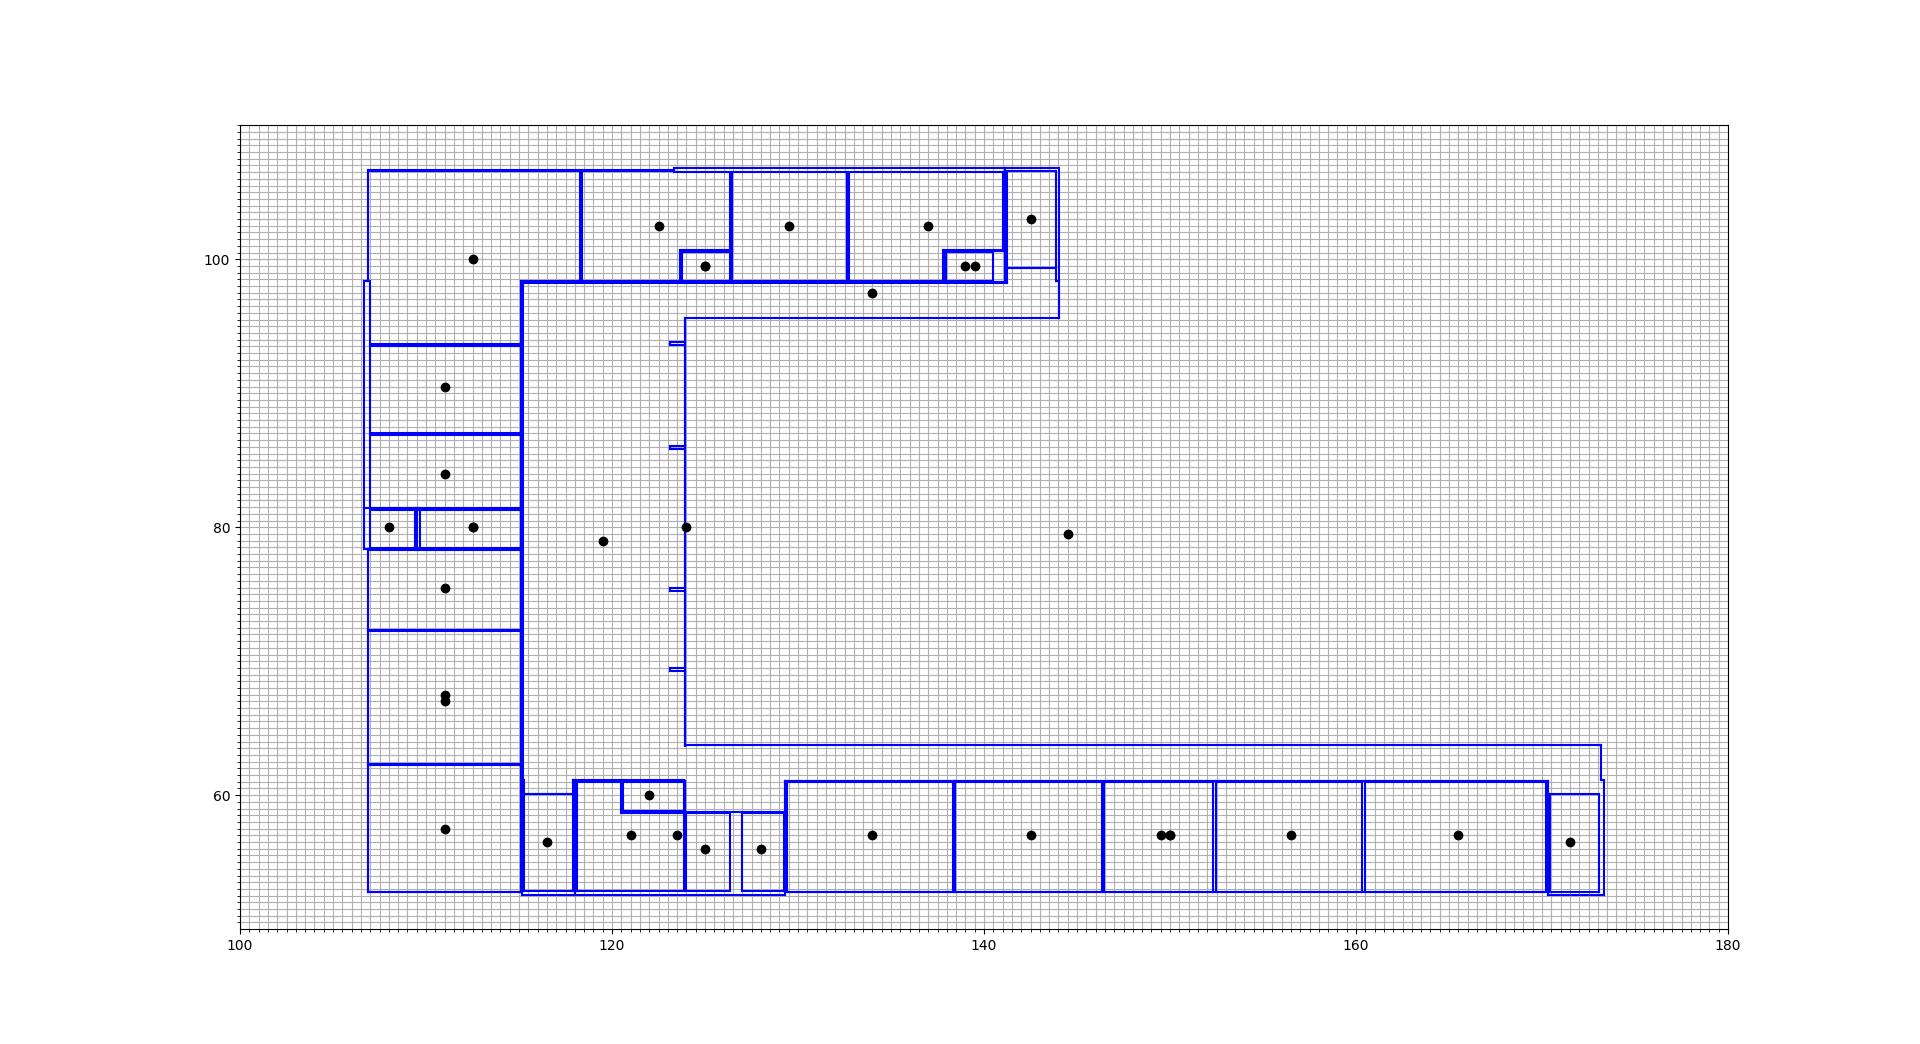
\includegraphics[width=1\textwidth]{fig/report/autogeneret_room_nodes.png}
    \label{}
    \caption[Design overview]{Example where it works somewhat well}
\end{figure}
This realisation would lead to another possible solution, namely doing convex decomposition of the rooms.


%One could achieve this by placing one room node in each room given that the rooms were convex. A convex polygon is defined by having any two nodes in the polygon being connected by a straight line without crossing the boundaries of the polygon. [show example of convex and non convex rooms] [insert reference]. The key word here is convex and for this approach to work the program would need to do a convex decomposition of all non convex rooms - which is to split a non convex polygon into convex sub polygons. Even though rooms in general are rectangle or square shaped and therefore convex, in practical applications it can be a bit complicated to do convex decomposition of non convex rooms.

%Another approach relies on the idea of generating more room nodes such that each room has multiple nodes that Spot has to visit. This would make the TSP solution slower and require Spot to walk a bit further. It would make up for it by being a much simpler method from an implementation standpoint and depending on how many nodes are being placed in each room, would still be a fairly robust solution. This was the approach that was chosen for this project. 

\subsection{Convex decomposition}
Convex decomposition of polygons is the idea of decomposing non convex rooms, to rooms that are convex. A convex polygon is a polygon where every node inside the polygon can be connect to every other node inside it with a straight line.

One solution was therefore to do convex decomposition of the rooms and place a room node at the center of each decomposed and convex room. 
The challenge with this solution was to decompose the rooms, which is the reason it in the end was not chosen as the final solution. The data did not allow for easy decomposition of the rooms, since the data is not very clean in the sense that there were a lot of lines and other things that made this approach difficult, see more in section [Data to work with].

The idea of placing optimal nodes were also an assumption that would have to be questioned and looked at from a different angle. Perhaps the best way to go about the problem would be to place a lot of room nodes and have a high probability that all corners and areas of the room would be covered. This was implemented using the K-means algorithm. 
Placing more nodes than optimal would make the TSP solution slower and require Spot to walk a bit further. It would make up for it by being a much simpler method from an implementation standpoint and depending on how many nodes are being placed in each room, would still be a fairly robust solution. This was the approach that was chosen for this project. 
%With this idea in mind the solution of doing clustering of the room nodes were chosen, more specifically the K-means algorithm.

%\subsection{K-means}
%The K-means algorithm was used to generate the room nodes.
%\begin{itemize}
%    \item Write that you are not finding the analytically best way to generate room nodes, but a discussion of this will be given in the discussion section.
%    \item The reason we need room nodes is not because we want the robot to take pictures at that spot but it is more that we want to make sure the robot visits certain areas or rooms. 
%\end{itemize}

As stated before, generating a complete room graph was needed to solve the TSP approximate solution therefore some kind of shortest path algorithm would have to be used to find the shortest distance between each of the room nodes. This shortest distance would be the weight of the edge between the nodes. There exist different shortest path algorithm but the go to standard is the A star algorithm since it is optimal and faster than many of the alternatives and it works well with grid based graph systems.

For one reason or another all the room nodes may not be connected to each other this would be due to some error with the data. Therefore before finding the shortest distance the program checks if there are room nodes that are not connected to the rest of the room nodes. If one or more of the room nodes are not connected to the rest of the room nodes these are removed.

With a complete room graph ready the program can now find the approximate TSP solution.

\begin{figure}[H]
    \centering
    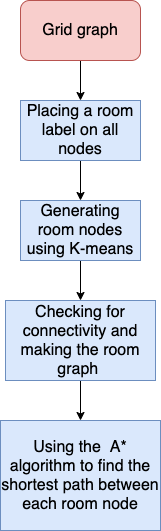
\includegraphics[width=0.3\textwidth]{fig/report/making_room_graph.png}
    \label{}
    \caption[Design overview]{}
\end{figure}



\section{TSP}
\begin{figure}[H]
    \centering
    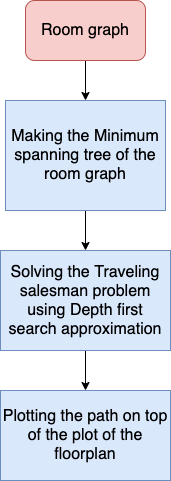
\includegraphics[width=0.3\textwidth]{fig/report/tsp_solution (1).png}
    \label{}
    \caption[Design overview]{}
\end{figure}
In this section the traveling salesman problem should be solved for the room graph. As mentioned earlier in the report an analytical solution is not needed in this case, and an approximate solution is sufficient for the purposes of this project. 
%There exist other algorithms but this one seemed to work fine.

Different approximate solution algorithms exist for TSP. A few parameters play a role when choosing which algorithm to go with. One parameter is how is the time performance, meaning how long will it take the program to run this algorithm. Another is how close to the optimal path will the solution be. The third thing to consider is how easy is the algorithm to implement given the frameworks and tools available to us.
Neither time nor performance are important factors in this program. Instead of spending a lot of time in analysis of the different algorithms and their theoretical constraints and performances the algorithm chosen in the end was chosen with ease of implementation in mind. %The 2-opt algorithm was chosen.
\begin{itemize}
    \item There are a lot of different approaches ant colony, nearest neighbour, christofides, 2-opt algorithm and others. The one went with was the 2-opt. Important that they run in polynomial time. The 2 opt is at most twice the optimal length while christofides is 1.5 optimal length, the 2 opt has shown to be around 5 \% better. Both could have been chosen, in this case I chose the 2-opt algorithm
\end{itemize}


The approximate solution used in this project is the 2-opt algorithm. 
A prerequisite of this algorithm is to have a graph that is complete, which was made sure of in the previous section.

As can be seen in \ref{TSP} the first step of the 2-opt algorithm is to make a minimum spanning tree of the graph. This is done using the Networkx library. 
The next step is to do a Depth first search traversal of the tree, again this is performed with the Networkx library. 
The final step of the 2-opt algorithm is to remove double vertices and connect the node to the next node in the tree. This is a bit more complex of a task, and the implementation of this is described in the implementation section \ref{2opt}

When the approximate solution for the room graph is found the path is transformed to the grid graph. The path information comes from doing the A star algorithm. The A star also includes the specific grid nodes traversed when finding the shortest distance from one room node to another room node. Therefore when finding the route between the room nodes this can be translated back to the grid graph. [Include figure that shows this]. This solution is then plotted on top of the plot of the floor plan, showing the final route.


\begin{itemize}
    \item how this problem is a bit different than the traditional tsp
\end{itemize}

